一条指令首先应该告诉机器,用户要干什么?例如加/减/乘/除或其他操作(\textbf{{由操作码实现}})。确定操作后就要知道对谁进行操作(\textbf{{由地址码实现}})。因此,一条指令应该由操作码和地址码两部分组成,如下图所示。

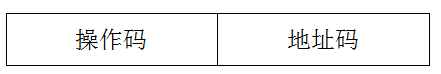
\includegraphics[width=2.08333in,height=0.35417in]{png-jpeg-pics/455DC55DE6F394CD8BD0B00DEFD79F74.png}

\textbf{操作码:}分为定长操作码和不定长操作码(也可称为扩展操作码或变长操作码)。一般将操作码放在每条指令的前一个字节或前多个字节,当读出操作码后就可以马上判定,这是一条零地址指令(如停机指令),还是单操作数指令(如求反、求补等操作),或者是双操作数指令(如加、减、乘、除等)。

\textbf{地址码:}有些书中将地址码称为操作数字段。\textbf{{下面分析地址码到底需要做什么。}}

\textbf{1)}需要指出操作数的地址,即用哪里的数来操作。

\textbf{2)}需要指出操作后的结果放在哪里,即给出结果存放的地址。

\textbf{3)}需要指出该条指令执行结束后怎么办,即需要指出下一条指令的地址。

\textbf{综上分析,}地址码应该指出操作数(一般称源操作数)的地址、运算结果需存放的地址、下一条指令的地址。由于操作数可以在主存,也可以在寄存器,因此以上所说的地址既可以是主存地址,也可以是寄存器地址,甚至还可以是I/O设备地址(I/O设备地址在第7章中介绍)。
